
\section{\label{sec:Ecological systems} Ecological systems}

In this section we will introduce the basic concepts and context of the
ecological systems that will be studied throughout the thesis.

\subsection{\label{sec:The Mass Mortality Event of Pinna nobilis} The Mass
  Mortality Event of \textit{Pinna nobilis}}

\subsection{\label{sec:Xylella fastidiosa: an emerging global
    threat}\textit{Xylella
    fastidiosa}: an emerging global threat}

\subsection{\label{sec:Coral reefs under threat} Coral reefs under threat}

\subsection{\label{sec:Ocean acidification} Ocean acidification}

\subsection{\label{sec:The decline of seagrass meadows} The decline of seagrass
  meadows}

\newpage
\section{\label{sec:Infectious disease modelling} Infectious
  disease modelling}

Infectious diseases are caused by pathogenic microorganisms, such as
bacteria, viruses, parasites, or fungi, when they invade other organisms, which
are called \textit{hosts} in this context. These pathogens proliferate inside
the host and can disrupt the normal functioning of the host organism by
damaging tissues, altering physiological processes, or triggering immune
responses that contribute to illness. Infectious diseases can affect a wide
variety of organisms, from plants and animals to humans, and they can spread
through various means, including direct interaction from infected individuals,
both by close contact or at a distance, or through vectors. Vectors are
organisms that transmit pathogens from one host to another, such as mosquitoes,
that usually are not affected by the disease themselves.

Modelling the spread of infectious diseases has a long history, with the first
mathematical model coming from the hand of Bernoulli in 1760
\cite{Bernoulli1760}, who developed a model to understand the spread of
smallpox. However, it was not until the early 20th century that we find the
foundation of the modern theory of infectious disease dynamics, with the
seminal work of Ronald Ross and Hilda P. Hudson
\cite{Ross1916,Ross1917,Ross1917_2} and Kermack and McKendrick
\cite{McKendrick}. Since then, a wide range of models have been
developed to understand the dynamics of infectious diseases and to predict
their spread. In general, these models can be classified into two main
categories: compartmental models and individual-based models.

\subsection{\label{sec:Compartmental models} Compartmental models}

Compartmental models are based on the assumption that the population can be
divided into different compartments or categories, each representing a
different state of the disease (e.g. susceptible to infection and infected).
Individuals move from one compartment to another following some dynamical
rules. Under the assumption of a well-mixed and sufficiently large population,
one can consider that  every pair of individuals has equal probability of
coming into contact with one another and that fluctuations in the number of
individuals in each compartment can be neglected. This is known as the mean
field approximation. Under these assumptions the dynamics of the disease can be
described by a set of differential equations that govern the transitions
between compartments.

\subsubsection*{\label{sec:The SIR model} The SIR model}

The most famous compartmental model is the SIR model, which is a simple
particular case of the general mathematical framework formulated by Kermack and
McKendrick \cite{McKendrick}. Because the original Kermack-McKendrick model
is quite general and complex, I will explain the SIR model following a more
modern and intuitive approach. The SIR model divides the population into three
compartments: susceptible individuals (S), infected individuals (I), and
recovered individuals (R). Individuals come into contact with each other at a
given rate $a$ and, in the case of a $S-I$ contact, the susceptible individual
becomes infected with a probability $b$. We assume that the incubation period
is short enough to be negligible; that is, a susceptible who contracts the
disease is infective right away. Infected individuals recover at a constant
rate $\gamma$, and once recovered, are assumed to be immune to the disease and
cannot be reinfected. We finally assume that there is no entry into or
departure from the population, no birth or natural deaths, so that
the population remains constant.

According to the mean field approximation, the probability that an infected
individual contacts a susceptible one is given by $a\cdot S/N$. Thus, the
average number of contacts between infected and susceptible individuals is
given by $a\cdot S/N\cdot I=a\cdot SI/N$. Finally, as the probability that a
susceptible individual becomes infected after a contact is $b$, the average
number of new infections will be given by the product of this probability and
average number of contacts between infected and susceptible individuals,
$b\cdot a\cdot SI/N=\beta SI/N$. These considerations lead to the following
description of the model given by a system of differential equations,
\begin{equation}\label{eq: normal_SIR_theo}
  \begin{array}{l}
    \dot{S}=-\beta SI/N          \\
    \dot{I}=\beta SI/N -\gamma I \\
    \dot{R}=\gamma I \ ,
  \end{array}
\end{equation}

Despite the aparent simplicity of the model, the non-linear nature of the
differential equations makes it difficult to find analytical solutions.
However, important quantitative insights can still be obtained by performing an
analytical study of the model. We will now derive some important results from
the SIR model, most of which cane be already found in reference
\cite{Murray_book}.

\subsubsection*{Conservation of the total population}

First let's start by the simplest insight: the assumption of population
conservation is inherently included in the model. We can prove this statement
by just adding the three differential equations in \cref{eq: normal_SIR_theo},
\begin{equation}
  \dot{S}+\dot{I}+\dot{R}=0\Longrightarrow S+I+R=\mathrm{const.}=N \ .
\end{equation}

Physicists usually call this kind of quantity a \textbf{conserved quantity}
or a \textbf{conservation law}. In this case, the conservation law has a
particular meaning: the total number of individuals in the population remains
constant, which was already assumed in the model. In general, conservation laws
can arise from other symmetries of the system and are not always so obvious. In
any case, these conserved quantities allow us to reduce the number of
independent variables in the system, which can be very useful to simplify the
analysis of the model. In this case, the conservation law allows us to reduce
the number of independent variables from three to two, so that we can study the
dynamics of the system in a two-dimensional phase space given by the variables
$S$ and $I$, as $R$ can be obtained from the relation $R=N-S-I$.

\subsubsection*{Threshold behaviour: the basic reproduction number}

Now consider the starting point of an epidemic, such our old friend the
COVID-19 pandemic. For sure at the beginning of the epidemic the number of
infectedindividuals is not zero, $I(0)>0$, while the number of recovered
individuals is indeed zero, $R(0)=0$. Thus, the number of susceptible
individuals at the beginning of the epidemic is $S(0)=N-I(0)$. If an epidemic
is to develop, the number of infected individuals must increase at the
beginning of the epidemic, but which are the conditions for this to happen?

Just by considering the differential equation for $I$ in \cref{eq:
  normal_SIR_theo} with our initial conditions we find the following
expression,
\begin{equation}\label{eq: threshold}
  \der{I}{t}\Big|\limitss{t=0}{}=I(0)\parentesi{\beta
    S(0)/N-\gamma}\Longrightarrow\left\{\begin{array}{l}
    \displaystyle\der{I}{t}\Big|\limitss{t=0}{}<0 \Longleftrightarrow
    S(0)<\frac{\gamma N}{\beta} \\\\
    \displaystyle\der{I}{t}\Big|\limitss{t=0}{}>0 \Longleftrightarrow
    S(0)>\frac{\gamma N}{\beta}
  \end{array}\right. \ \ .
\end{equation}

The condition \cref{eq: threshold} defines a threshold for the developing of an
epidemic in the $SIR$ model! This is, there is a critical number of susceptible
individuals below which the epidemic will not develop,
\begin{equation}
  S_c=\frac{\gamma N}{\beta}\equiv \rho \ .
\end{equation}

The critical parameter $\rho$ is sometimes called the \textit{relative removal
  rate} and its reciprocal, $\sigma=\beta/(\gamma N)$, the \textit{infection’s
  contact rate}. This threshold behaviour can be further simplified by
considering the so-called \textit{basic reproduction number}, $R_0$, defined
as,
\begin{equation}
  R_0=\frac{S(0)}{\rho}=S(0)\sigma=\frac{\beta S(0)}{\gamma
    N}\simeq\frac{\beta}{\gamma} \ ,
\end{equation}
in which we have considered that $S(0)\simeq N$ at the beginning of the
epidemic.

The basic reproduction number is a very important quantity in
epidemiology, an it can be proved that it measures the average number of
secondary infections given by a primary infection in a \textit{fully
  susceptible population}. To see it we just need to recall the definition of
the rates and ``read'' the expression. $\beta S(0)/N$ is the rate of new
infections produced by a primary infection (as we are at time $t=0$). In other
words, $\beta	S(0)/N$ is the number of secondary infections produced by a
primary infection \textit{per unit time}. Finally, we observe that, as $\gamma$
is the rate of recovery of infected individuals, $1/\gamma$ is the average time
an individual remains infected. The product of the number of secondary
infections produced by a primary infection per unit time and the average time
an infected individual remains infected gives the total number of secondary
infections produced by a primary infection in the whole susceptible population.
Voilà! This is nothing but the basic reproduction number, $R_0$.

It can be more formally proved that this quantity defines a threshold for the
development of an epidemic from the fact that $S$ is a monotonically decreasing
function, which implies $S(t)<S(0) \ \forall t>0$.
\begin{equation}\label{eq: threshold_t}
  \der{I}{t}=I\parentesi{\beta S-\gamma}\leq I\parentesi{\beta
    S(0)-\gamma}=\gamma I\parentesi{\frac{S(0)}{\rho}-1}=\gamma
  I\parentesi{R_0-1} \
  ,
\end{equation}
so that for $R_0<1$, $\dot{I}<0 \ \forall t>0$ and thus $I(0)>I(t)$ as
$t\to\infty$, which basically means that the epidemic dies out, while for
$R_0>1$ the epidemic grows.

This threshold behaviour agrees with our intuition given the definition of
the basic reproduction number: if a primary infection produces more than 1
secondary infection an epidemic will develop, while if it does not reach to
infect at least one individual it will die out. Furthermore, note that
because of our mean field approach, the number of secondary infections produced
by a primary one refers to the \textit{average} number of secondary
infections.

\subsubsection*{Initial phase approximation}

An approximated closed analytical result can be obtained by considering the
initial phase of the epidemic, when the number of infected individuals is small
compared to the number of susceptible individuals, $I\ll S$. In this case, the
number of susceptible individuals is approximately the total population,
$S\approx N$, as the number of recovered individuals is negligible,
$R\approx0$. Under these conditions, the dynamics of the infected population
can be described by the following differential equation,
\begin{equation}
  \der{I}{t}=\beta S/N I-\gamma I\approx\beta I-\gamma I=(\beta-\gamma)I \ ,
\end{equation}
which has the solution,
\begin{equation}
  I(t)=I(0)e^{(\beta-\gamma)t}=I(0)e^{\gamma(R_0-1)t} \ .
\end{equation}

This result shows that the number of infected individuals grows exponentially
at the beginning of the epidemic, with a growth rate related to $R_0$.
This approximation is very useful to understand the initial phase of the
epidemic, when the number of infected individuals is small, but it is only
valid and useful for short times after the beginning of the epidemic.

In \cref{fig: SIR_model}(a) we show the numerical solution of the SIR model for
a given set of parameters. The fraction of susceptible, infected, and recovered
population is shown as function of time. The black dashed line represents the
initial phase approximation of the model, which is in good agreement with the
numerical solution of the model at the beginning of the epidemic. In the inset,
we can see that the initial growth of the epidemic is indeed exponential
(a straight line in log-linear scale), as predicted by the model.

\subsubsection*{Maximum number of infected individuals}

Another important analytical result that can be obtained from this model is
the maximum of infected individuals, that gives an idea of how severe the
epidemic will be. To find this maximum we just need to find the maximum of
$I(t)$, which is given by the condition $\dot{I}=0$. From the differential
equation for $I$ in \cref{eq: normal_SIR_theo} we find the following relation,
\begin{equation}
  \der{I}{t}=0\Longrightarrow\beta S/N-\gamma=0\Longrightarrow
  S=\frac{\gamma N}{\beta}=\rho \ .
\end{equation}

So the maximum of infected individuals, given the development of a proper
epidemic, will take place when $S(t)=\rho$. But we still don't know the
maximum number of infected individuals. To do so, we first need to go through
a smart mathematical trick. Dividing the differential equations for $S$ and $I$
(considering $I\neq0)$) we obtain,
\begin{equation*}
  \frac{\dif I}{\dif S}=-1+\frac{\gamma}{\beta S}=-1+\rho/S \quad (I\neq0) \
  .
\end{equation*}

Integrating the relation,
\begin{equation*}
  \int_{I(0)}^{I}\dif I=\int_{S(0)}^S\dif S \keys{-1 + \rho/S} \Longrightarrow
  I-I(0)=S(0)-S+\rho\ln(\frac{S}{S(0)}) \ ,
\end{equation*}
we obtain the phase plane trajectories for $S$ and $I$ given by,
\begin{equation}\label{eq: max_I_eq}
  I+S=I_0+S_0+\rho\ln(\frac{S}{S(0)})=N+\rho\ln(\frac{S}{S(0)}) \ ,
\end{equation}
where we have considered $I(0)+S(0)=N$ given that $R(0)=0$.

Note that \cref{eq: max_I_eq} can be rewritten as
$I+S-\rho\ln(S)=N-\rho\ln(S_0)=\mathcal{C}$, so that the right-hand side of the
equation is a constant. This means that we have just found another conservation
law for the system! This one is not so obvious as the previous one, but it is
still a very useful result. In essence, we now can describe the dynamics of the
system with only one independent variable, $S$, as $I$ can be obtained from the
relation in \cref{eq: max_I_eq}.

Finally we find an expression for the maximum of infected individuals by
substituting the condition previously found (the maximum occurs when
$S(t)=\rho$)
in \cref{eq:  max_I_eq},
\begin{equation}
  I(t)=N+\rho\ln{\frac{S(t)}{S(0)}}-S(t) \Longrightarrow
  I_{max}=N+\rho\claudator{\ln(\frac{\rho}{S_0}) -
    1}=N+\frac{S(0)}{R_0}\claudator{\ln(\frac{1}{R_0}) - 1} \ .
\end{equation}

In \cref{fig: SIR_model}(b) we can see how the analytical result compares with
the numerical solution of the model for different values of $R_0$.

\begin{figure}[H]
  \centering
  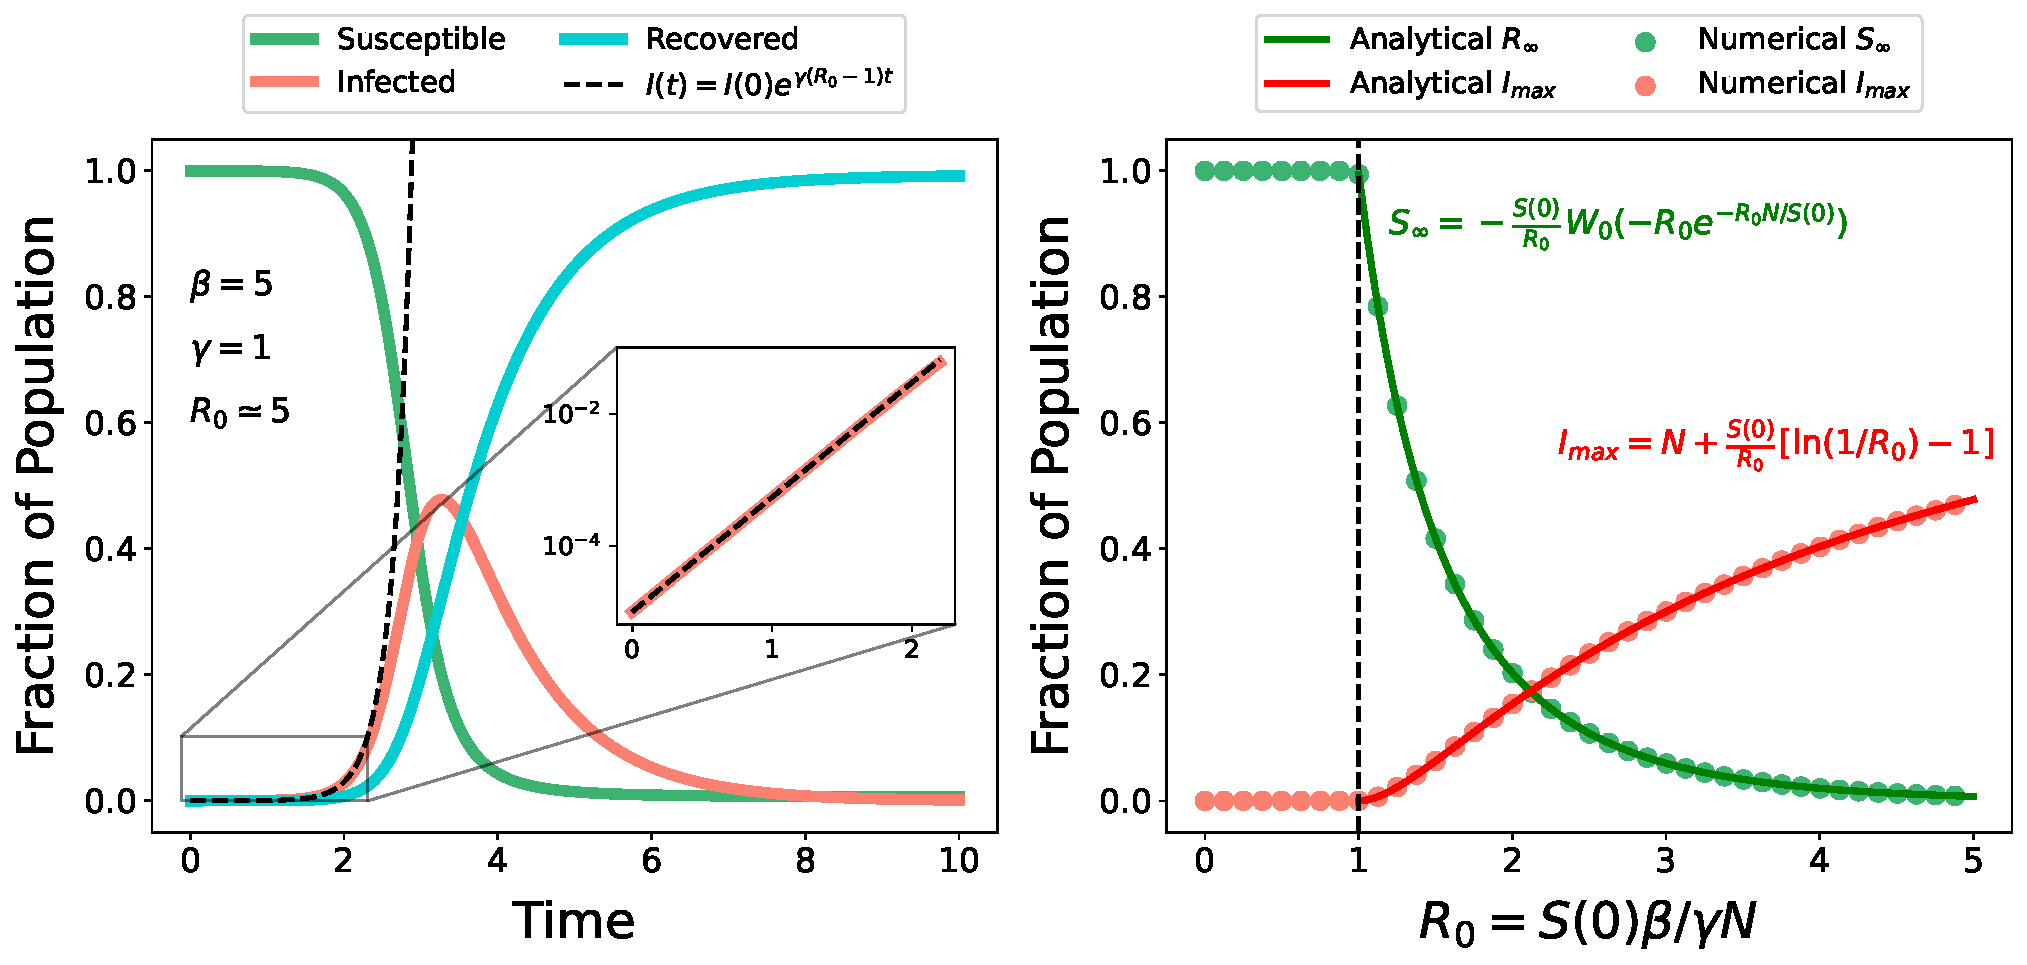
\includegraphics[width=1\textwidth]{Figures/SIR_model_analysis.pdf}
  \caption[Numerical and analytical analysis of the SIR model.]{\label{fig:
      SIR_model} \textbf{Numerical and analytical analysis of the SIR model.}
    (a) Numerical solution of the SIR model for a given set of parameters. The
    fraction of susceptible (green), infected (red), and recovered (blue)
    population is shown as function of time. The black dashed line represents
    the initial phase approximation of the model. (b) Comparison between the
    analytical results obtained from the SIR model and the numerical solution
    of the model for different values of $R_0$. The maximum number of infected
    individuals, $I_{max}$, and the final number of susceptible individuals,
    $S_{\infty}$, are shown as function of the basic reproduction number,
    $R_0$. The analytical results are in good agreement with the numerical
    solution of the model.
  }
\end{figure}

\subsubsection*{Final number of susceptible individuals}

Similarly we can find the final number of susceptible individuals at the end
of
the epidemic, for sure a very important quantity. By dividing the
differential
equations for $S$ and $R$, we obtain,
\begin{equation*}
  \frac{\dif S}{\dif R} = -\frac{\beta}{\gamma}S=-\frac{S}{\rho}
  \Longrightarrow\int_{S(0)}^S\frac{\dif
    S}{S}=-\frac{1}{\rho}\int_{R(0)=0}^R\dif
  R\Longrightarrow\ln(\frac{S}{S(0)})=-\frac{R}{\rho} \ .
\end{equation*}

As $I(\infty)=0$, necessarily $R(\infty)=N-S(\infty)$ so that we get the
following expression for the final number of susceptible individuals,
\begin{equation}\label{eq: trascendental_S_inf}
  S(\infty) - \rho\ln(S(\infty))=N-\rho\ln(S(0)) \ .
\end{equation}

$S(\infty)$ is nothing but the positive root of the transcendental equation
\cref{eq: trascendental_S_inf}. In fact, this transcendental equation can be
solved by means of the Lambert's $W$ function \cite{Lethonen2016},
\begin{equation}
  S(\infty)=-\rho\cdot W_0\claudator{-\frac{S(0)}{\rho} \,
    e^{-N/\rho}}=-\frac{S(0)}{R_0}\cdot W_0\claudator{-R_0 \, e^{-R_0N/S(0)}} \
  .
\end{equation}

Of course, given that $N=S+I+R$ and $I(\infty)=0$, we can obtain the final
number of recovered individuals as $R(\infty)=N-S(\infty)$. In \cref{fig:
  SIR_model}(b) we show how the analytical result compares with the numerical
solution of the model for different values of $R_0$.

\begin{remark}
  Note that all the analytical results that we have obtained can be expressed
  as function of the initial conditions of the system (e.g. $S(0)$) and the
  basic reproduction number, $R_0$. This is a very important result, as it
  allows us to understand and predict the dynamics of the whole system by just
  knowing, in essence, the basic reproduction number.
\end{remark}

% The Lambert's $W_l(x)$ function is bivalued for $x\in(-1/e,0)$, so that it is
% necessary to choose a branch for such values of $x$. In this epidemiological
% context it has been already shown that the branch $l=0$ has to be chosen when
% $S(t)<S_c$ \cite{Rodri_thesis}, and clearly $S_\infty<S_c$. With this analysis
% we ensure that the final number of susceptible individuals is a strictly
% positive number, $S_\infty>0$, given the properties of the Lambert's
% function.

So far we have shown how, under minimal assumptions, one can build an epidemic
model such as the SIR model. In addition, we have shown how to obtain some
important analytical results from the model, such as the threshold for the
development of an epidemic, i.e. the \textit{basic reproduction number}; the
maximum number of infected individuals, and the final number of susceptible
individuals. However, the SIR model is one of the simplest compartmental
models, and more complex models have been developed to account for more
realistic scenarios. For such models, analytical results are usually not
available, and numerical simulations are required to understand the dynamics of
the diseases they describe. Fortunately, there are a couple of formal
approaches that can be used to derive the basic reproduction number of
basically any compartmental model: linear stability analysis and the next
generation matrix approach.

\subsection{Linear stability analysis}

Linear stability analysis is a powerful tool that can be used to study the
dynamics of a \textbf{dynamical system} around its \textbf{fixed points}. The
basic idea is to linearize the system of differential equations around these
equilibrium points and study the stability of the system by analysing the
\textbf{eigenvalues} of the \textbf{Jacobian} of the system. A
\textit{dynamical system} is a system that evolves over time,
such as the SIR model. The \textit{fixed points} of the system are the points
where it does not change over time, i.e. the points where the derivatives of
the variables of the model are zero. The \textit{Jacobian} of the system is a
matrix that contains the first-order partial derivatives of the variables of
the system. The \textit{eigenvalues} of the Jacobian matrix are the roots of
the characteristic polynomial of the matrix, obtained through the equation
$\det(J-\lambda I)=0 $, and they determine the stability of the system. If the
real part of all the eigenvalues is negative, the system is stable, while if
the real part of at least one eigenvalue is positive, the system is unstable.
Let's see how this works in practice.

For the SIR model, the fixed points are given by the condition
$\dot{S}=\dot{I}=\dot{R}=0$, which implies $I=0$ with any value of $S$ and $R$.
Thus, the fixed points of the system are given by $(S^*,I^*,R^*)=(S,0,N-S)$.
These fixed points are also called \textit{disease-free} state of the system,
as the number of infected individuals is zero. The Jacobian matrix of the
system is given by,
\begin{equation}
  J=\begin{pmatrix}
    \partial\dot{S}/\partial S & \partial\dot{S}/\partial I &
    \partial\dot{S}/\partial R                                \\
    \partial\dot{I}/\partial S & \partial\dot{I}/\partial I &
    \partial\dot{I}/\partial R                                \\
    \partial\dot{R}/\partial S & \partial\dot{R}/\partial I &
    \partial\dot{R}/\partial R
  \end{pmatrix}=\begin{pmatrix}
    -\beta I/N & -\beta S/N       & 0 \\
    \beta I/N  & \beta S/N-\gamma & 0 \\
    0          & \gamma           & 0
  \end{pmatrix} \ ,
\end{equation}

Now we substitute the fixed point in the Jacobian matrix and we obtain,
\begin{equation}
  J=\begin{pmatrix}
    0 & -\beta S^*/N       & 0 \\
    0 & \beta S^*/N-\gamma & 0 \\
    0 & \gamma             & 0
  \end{pmatrix} \ .
\end{equation}

The eigenvalues of the Jacobian matrix are the roots of the characteristic
polynomial of the matrix, which is given by $\det(J-\lambda I)=0$. In this case
the characteristic polynomial is given by,
\begin{equation}
  \det(J-\lambda I)=\begin{vmatrix}
    -\lambda & -\beta S^*/N                & 0        \\
    0        & \beta S^*/N-\gamma -\lambda & 0        \\
    0        & \gamma                      & -\lambda
  \end{vmatrix}=\lambda^2(\beta S^*/N-\gamma-\lambda) \ .
\end{equation}

The roots of the characteristic polynomial are given by $\lambda_1=\lambda_2=0$
and $\lambda_3=\beta S^*/N-\gamma$. As we have previously stated, the stability
of the system is determined by the real part of these eigenvalues. Of course,
the eigenvalues $\lambda_1$ and $\lambda_2$ are zero, so they do not provide
any information about the stability of the system.

The eigenvalue $\lambda_3$ is negative if $\beta S^*/N<\gamma$, thus meaning
that the fixed point $(S^*,I^*,R^*)$ is stable if this condition is satisfied.
On the other hand, the fixed point is unstable if $\beta S^*/N>\gamma$. Indeed,
this conditon defines the basic reproduction number, $R_0$, as we can rewrite
the condition for the stability of the fixed point as $R_0=\beta S^*/\gamma N$
greater or smaller than 1.

% Comment on the conserved quantities that can be already observed from the Jacobian matrix.
Finally note that the Jacobian matrix also provides us with another important
insight about the system: the presence of conserved quantities. In this case,
the sum of the first and third rows of the Jacobian matrix is zero, which
indicates that the system has two conserved quantities, which we have already
found: the total number of individuals in the population and \cref{eq:
  max_I_eq}.

\begin{remark}
  The stability of the fixed points of a dynamical system can be determined by
  analysing the eigenvalues of the Jacobian matrix of the system. If the real
  part of all the eigenvalues is negative, the fixed point is stable, while if
  the real part of at least one eigenvalue is positive, the fixed point is
  unstable. In epidemic models the basic reproduction number, $R_0$, determines
  the	stability of the disease-free states of the system, which are the fixed
  points where the number of infected individuals is zero. If $R_0<1$, the
  fixed points are stable, while if $R_0>1$, the fixed points are unstable.
  The basic reproduction number is a threshold for the development of an
  epidemic: if $R_0<1$, the epidemic will die out, while if $R_0>1$, the
  epidemic will propagate. In addition, the Jacobian matrix of the system
  provides us with important insights about the system, such as the presence of
  conserved quantities.
\end{remark}

\subsection{The next generation matrix method}
We have previously shown that the basic reproduction number, $R_0$ of a
compartmental model can be obtained by analysing the stability of the fixed
points corresponding to the disease-free state of the model. Specifically, the
basic reproduction number, $R_0$, is related to the largest non-zero eigenvalue
of a fixed point, $\Lambda$, such that $R_0>1$ if $\Lambda>0$. However, the
Jacobian matrix of a compartmental model can be quite large and complicated, so
the derivation of the basic reproduction number following this method can be
cumbersome. The next generation matrix method is an ingenious method that can
be used to derive the basic reproduction number of any compartmental model
directly, without the need to analyse the stability of the fixed points. We
will make use of this method in \cref{part:nacras,part:VBD} of this thesis.

In the NGM method, $R_0$ is identified as the dominant eigenvalue of a suitably
defined linear operator (a linear matrix in a suitable basis). This operator is
obtained by decomposing the Jacobian of the infected/infecting compartments
evaluated at the disease-free state,  $J^*$, in the form $J=T+\Sigma$, where
$T$ is the \textit{transmission part}, that describes the production of new
infections, and $\Sigma$  the \textit{transition part}, that describes changes
of state. Then, it can be proved \cite{Diekmann2010} that the \textit{basic
  reproduction number} $R_0$ is given by the spectral radius (i.e. the largest
eigenvalue) of the next generation matrix, $K$, defined as,
\begin{equation}
  R_0=\rho(K) \quad \textrm{with} \quad K=-T\Sigma^{-1} \
\end{equation}

\begin{theorem}[The next generation matrix method]
  \small\sffamily
  Steps of the next generation matrix:
  \begin{enumerate}
    \item Compute the Jacobian matrix of the infected/infecting compartments of
          the model evaluated at the disease-free state, $J^*$.
    \item Decompose the Jacobian matrix in the form $J^*=T+\Sigma$, where $T$
          is
          the transmission part and $\Sigma$ the transition part.
    \item Compute the inverse of the transition part, $\Sigma^{-1}$.
    \item Compute the next generation matrix, $K=-T\Sigma^{-1}$.
    \item Solve the characteristic equation $\det(K-\lambda I)=0$ to obtain the
          eigenvalues of the next generation matrix.
    \item Obtain the basic reproduction number, $R_0$, as the largest
          eigenvalue of the next generation matrix.
  \end{enumerate}
\end{theorem}

To appreciate the power of the NGM method, let's see how it can be applied to a
slightly more complex model than the SIR model. We will now consider a
compartmental model for vector-borne plant diseases.

\subsubsection*{A compartmental model for vector-borne plant diseases}

The simplest way to do this is to consider a compartmental model with five
compartments: susceptible individuals ($S$), infected individuals ($I$),
recovered individuals ($R$), susceptible vectors ($S_v$), and infected vectors
($I_v$). For most vector-borne plant diseases, we can assume that the only
mechanism of disease spread is the direct transmission from infected vectors to
susceptible plants at a given rate $\alpha$. Infected individuals recover at
a rate $\gamma$. The total number of plants is given by $N$, and the total
number of vectors is given by $N_v$. Vectors are assumed to be born at a
constant rate $\delta$ proportional to the total number of vectors and die at a
constant rate $\mu$. With these assumptions, the dynamics of the disease can be
described by the following system of differential equations,
\begin{equation}\label{eq: SIRV_model}
  \begin{array}{l}
    \dot{S}=-\beta SI_v/N_v                       \\
    \dot{I}=\beta SI_v/N_v -\gamma I              \\
    \dot{R}=\gamma I                              \\
    \dot{S_v}=\delta N_v -\alpha S_vI/N - \mu S_v \\
    \dot{I_v}=\alpha S_vI/N-\mu I_v \ ,
  \end{array}
\end{equation}

We can easily check that the plant population is conserved by adding the
differential equations for $S$, $I$, and $R$,
\begin{equation}
  \dot{S}+\dot{I}+\dot{R}=0\Longrightarrow S+I+R=N \ .
\end{equation}

Similarly, to check if the vector population is conserved we add the
differential equations for $S_v$ and $I_v$,
\begin{equation}
  \dot{S_v}+\dot{I_v}=\delta N_v -\mu S_v -\mu I_v=0\Longrightarrow
  N_v(\delta-\mu)=0 \ .
\end{equation}

This equation implies that the vector population is conserved only if
$\delta=\mu$, which is a reasonable assumption given that the birth and death
rates of vectors are usually similar. By now, this is the case we will
consider in the following analysis, but we will see in \cref{part:VBD}
that thinks can get really complicated if we relax this assumption.

After this initial check, we can proceed to obtain an expression for the basic
reproduction number, $R_0$. To compute it we can follow the next generation
matrix approach. We first need to identify the disease-free state of the
system, which is given by $(S^*,I^*,R^*,S_v^*,I_v^*)=(S(0),0,N-S(0),N_v,0)$.
Then we need to write down the Jacobian matrix of the subsystem corresponding
to the infected/infecting compartments, $I$ and $I_v$ in this case and evaluate
it at the disease-free state. This matrix is given by,
\begin{equation}
  J=\begin{pmatrix}
    \partial \dot{I}/\partial I   & \partial \dot{I}/\partial I_v   \\
    \partial \dot{I_v}/\partial I & \partial \dot{I_v}/\partial I_v
  \end{pmatrix}=
  \begin{pmatrix}
    -\gamma      & \beta S/N_v \\
    \alpha S_v/N & -\mu
  \end{pmatrix}=
  \begin{pmatrix}
    -\gamma      & \beta S(0)/N_v \\
    \alpha N_v/N & 0
  \end{pmatrix} \ ,
\end{equation}
where we have substituted the fixed point
$(S^*,I^*,R^*,S_v^*,I_v^*)=(S(0),0,N-S(0),N_v,0)$ in the last step.

Next we decompose the matrix in the transmission and transition parts,
$J=T+\Sigma$, and compute the inverse of the transition part, $\Sigma^{-1}$,
\begin{equation}
  T=\begin{pmatrix}
    0 & \beta S(0)/N_v \\
    0 & 0
  \end{pmatrix} \quad \text{and} \quad
  \Sigma=\begin{pmatrix}
    -\gamma      & 0    \\
    \alpha N_v/N & -\mu
  \end{pmatrix} \quad \Longrightarrow \quad
  \Sigma^{-1}=\frac{-1}{\gamma\mu}\begin{pmatrix}
    \mu          & 0      \\
    \alpha N_v/N & \gamma
  \end{pmatrix} \ .
\end{equation}

We finally obtain the next generation matrix, $K$, as the product of the
transmission and transition parts,
\begin{equation}
  K=-T\Sigma^{-1}=\frac{1}{\gamma}\begin{pmatrix}
    \frac{\beta\alpha}{\gamma\mu}\frac{S(0)}{N} &
    \frac{\beta}{\mu}\frac{S(0)}{N}                 \\
    0                                           & 0
  \end{pmatrix} \ .
\end{equation}

The basic reproduction number, $R_0$, is given by the spectral radius of the
next generation matrix, $K$, which is the largest eigenvalue of the matrix. In
this case, the matrix is a $2\times2$ matrix, so the eigenvalues can be easily
obtained. The characteristic polynomial of the matrix is given by,
\begin{equation}
  \det(K-\lambda I)=\begin{vmatrix}
    \frac{\beta\alpha}{\gamma\mu}\frac{S(0)}{N}-\lambda &
    \frac{\beta}{\mu}\frac{S(0)}{N}                                \\
    0                                                   & -\lambda

  \end{vmatrix}=\lambda\parentesi{\lambda-\frac{\beta\alpha}{\gamma\mu}
    \frac{S(0)}{N}}
  \ ,
\end{equation}
so the eigenvalues are $\lambda_1=0$ and $\lambda_2=\beta\alpha S(0)/(\gamma\mu
  N)$. The basic reproduction number, $R_0$, is given by the largest eigenvalue
of the matrix, so
\begin{equation}
  R_0=\frac{\beta\alpha S(0)}{\gamma\mu N} \ .
\end{equation}

\subsection{\label{sec:Individual-based models} Individual-based models}

Individual-based models describe the dynamics of infectious diseases by
considering the individuals of the population as discrete entities that can
interact with each other. These models are particularly useful when the
population is not well-mixed, the interactions between individuals are
heterogeneous, the individuals can not be considered as identical or when an
spatial setting is considered. In individual-based models, the dynamics of the
disease are described by stochastic processes that govern the interactions
between individuals. These models are usually more complex than compartmental
models, so that analytical results are not usually available, but they can
provide more realistic insights into the dynamics of infectious diseases.

In individual-based models the population is represented by a set of
individuals, each of which can be in different \textbf{states}. More formally,
the \textbf{system} at time $t$ is defined by the set of states of the
individuals in the population at that time. The states of the individuals can
change over time according to \textbf{events} that occur in the system, whcih
consequently change the state of the system. These events can be triggered by
the interactions between individuals, the environment, internal or other
external factors. The events are characterized by their \textbf{rates}, which
determine the probability of occurence per unit time. Mathematically, the
dynamics of the system are described by the \textbf{master equations}
\cite{Toral_master_eqs}, which are a set of differential equations that
describe the probability of the system being in a given state at a given time.
The master equations are usually difficult to solve analytically, so numerical
methods are used to simulate the dynamics of the system.

\subsubsection*{The Gillespie algorithm}

There are several ways to simulate the dynamics of individual-based models, but
one of the most common methods is the Gillespie algorithm \cite{Gillespie1977},
which is indeed an exact and unbiased algorithm to simulate stochastic
processes. The Gillespie algorithm is based on the idea that the system will
remain in a given state for a random amount of time until an event occurs,
which will then change the state of the system. Thus, the change of state of
the system can determined by two independent random processes: the time to the
next event and the particular event that occurs.

Consider that we are simulating a system with $M$ possible events, each of
which has a rate $w_i$ of occurence. The time of the next event is given by
\begin{equation}
  t_{\textrm{next}}=\frac{-\ln(r_1)}{W} \ ,
\end{equation}
where $W=\sum_i^M w_i$ is the total rate of any event happening and
$r_1=\hat{\mathbb{U}}(0,1)$ is a distributed random number in the interval
$[0,1]$.

Once the time of the next event has been computed, we choose the event to
implement according to their conditional probabilities $p_i=w_i/W$. Basically,
we draw another uniformly distributed random number $r_2$ and compare it to
these conditional probabilities, finding the smallest $i$ satisfying
$\sum_i^Mp_i>v$. The system is then updated according to the chosen event and
the time is updated to $t_{\textrm{next}}$. This process is repeated until a
termination condition is met. In \cref{alg:gillespie} we show a pseudocode
implementation of the Gillespie algorithm.

\begin{algorithm}
  \caption{Gillespie Algorithm}
  \label{alg:gillespie}
  \begin{algorithmic}[1]
    \State Initialize time $t \gets 0$, and set the initial state of the
    system.
    \While{termination condition is not met}
    \State Calculate the propensity functions $w_i(t)$ for all possible
    events $i$.
    \State Calculate the total propensity $W(t) = \sum_i^M w_i(t)$.
    \State Generate two random numbers $r_1$ and $r_2$ uniformly
    distributed in $[0,1]$.
    \State Calculate the time until the next reaction event $\tau =
      \frac{-\ln(r_1)}{W(t)}$.
    \State Select the next reaction $j$ according to the probabilities
    $P(j) = \frac{w_j(t)}{W(t)}$ compared to $r_2$.
    \State Update the system state according to the chosen reaction.
    \State Update time $t \gets t + \tau$.
    \EndWhile
  \end{algorithmic}
\end{algorithm}

The Gillespie algorithm provides a statistically exact way to solve the
master equations underlying the IBM and gives a physical sense to the simulated
time, as it comes directly from the event rates. However, one of its major
drawbacks is the computational expense of the algorithm. Nevertheless, some
tricks can be implemented to overcome these limitations and still provide an
exact solution to the stochastic process. Two tricks have been used in our
implementation of the Gillespie algorithm of \cref{ch:nacras_II}: first,
instead of comparing $p_i$ with the random number $r_2$ we use $w_i$ over
$v\cdot W$, as this way only a product is computed (instead of $M$)
\cite{Toral_master_eqs}; second, we implemented the sorting direct method
\cite{MCCOLLUM200639}. The method consists in dynamically sorting the events
and try to apply the most frequent ones first, which can save a considerably
amount of computational time. In \cref{alg:Chose_apply_event} we show a
pseudocode implementation of core of the numerical method.

\begin{algorithm}[H]
  \caption{Sorting direct method}
  \label{alg:Chose_apply_event}
  \begin{algorithmic}[1]

    \State U = rand() * W \Comment{Random number multiplied by
      total rate}

    \For {$i=1,\ldots,M$} \Comment{Iterate over events}

    \If {U $<$ sum(rates[orders[1:i]])}

    \State events[i](*args) \Comment{Execute corresponding event}\\

    \If {i != 1} \Comment{Sort reactions array}

    \State aux\_e = copy(events)
    \State aux\_o = copy(orders)\\

    \State events[i-1] = aux\_e[i]
    \State events[i] = aux\_e[i-1]\\

    \State orders[i-1] = aux\_o[i]
    \State orders[i] = aux\_o[i-1]

    \EndIf

    \State break

    \EndIf

    \EndFor

  \end{algorithmic}
\end{algorithm}

\AG{Something that could be added here is an example of the SIR model
  implemented with the Gillespie algorithm. We could also show how the mean
  field approximation works, both analytically and numerically.}

We have seen how mathematical models can be used to study the dynamics of
infectious diseases, which can provide important insights into the spread of
diseases \textit{at a local level}. However, another important aspect of
infectious diseases is their spread and establishment \textit{at a global
  level}. In the following section, we will discuss the most common methods
used to study the potential distribution of diseases and their limitations,
particularly in a context of climate change.

\section{\label{sec:Disease biogeography} Disease biogeography}

Biogeography is the study of the distribution of species and ecosystems across
the Earth's surface, and it is a fundamental field in ecology. Disease
biogeography is a subfield of biogeography that focuses on the geographical
distribution of infectious diseases and the factors that influence their
establishment, such as climate, land use, human activities, and the presence of
vectors or reservoirs. Understanding how these factors influence the
spread of diseases at a geographical scale is essential to predict the
risk of emergent diseases developing in new areas. This, in turn, can help
public health authorities to design effective strategies to prevent and control
the spread of diseases.

The study of disease biogeography is particularly challenging due to the
complexity of the interactions between the environment, the pathogens, the
vectors, and the hosts involved in the disease transmission cycle. The
potential distribution of diseases has been mostly studied using correlative
species distribution models, which link presence and absence data of diseases
to environmental variables based on correlative methods. Despite their wide
use, these models have several limitations, both conceptual and practical. In
this section, we will briefly review the main concepts of biogeography and
explain the basic principles of species distribution models. Finally, we will
discuss how the limitation of using this framework to study the potential
distribution of infectious diseases.

% Ecological niche concept
\subsection{\label{sec:Ecological niches} Ecological niches}

The concept of ``ecological niche'' is central to the study of biogeography,
but it has evolved significantly since its inception. The term "niche" was
first introduced by Grinnell in 1917 to describe the set of environmental
conditions within a species' range that dictate its distribution
\cite{Grinnell1917}. This is, the niche of a species is the set of
environmental conditions, such as temperature, humidity, and precipitation,
that are suitable for the species to survive and reproduce. This early
interpretation, known as the Grinnellian niche, emphasized the abiotic factors
essential for the survival and distribution of species, but neglected the
biotic interactions that also shape species' distributions. Indeed, some years
later Charles S. Elton redefined the niche concept to encompass the roles
species play within an ecosystem, including their interactions with other
species. This Eltonian definition shifted the focus towards the biotic aspects
of ecological niches \cite{Elton1927}.

\begin{figure}[H]
  \centering
  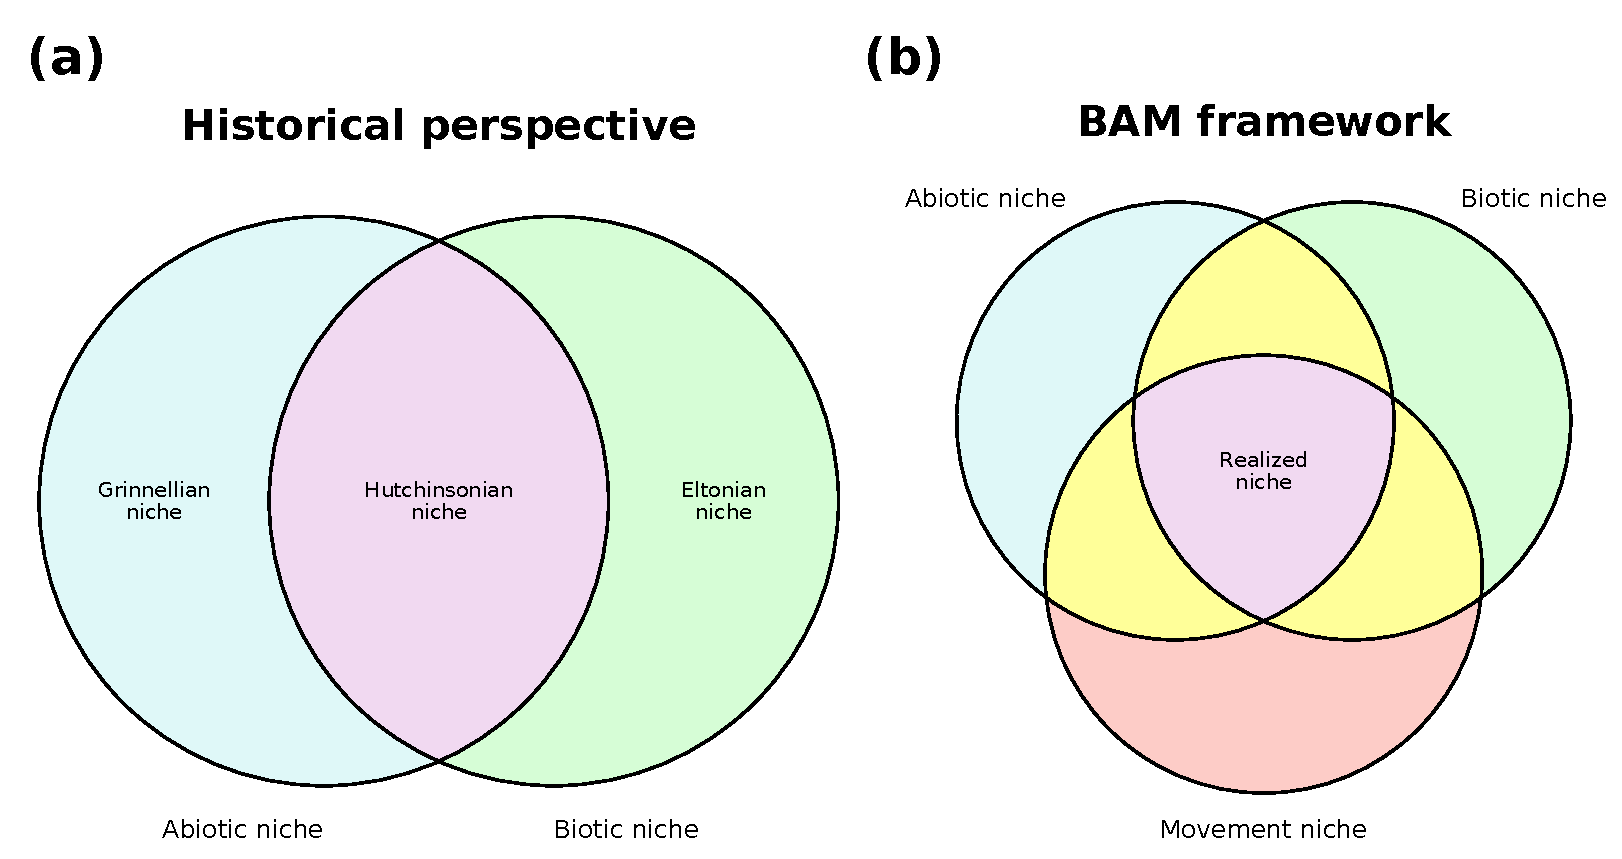
\includegraphics[width=1\textwidth]{Figures/Niche_theory.pdf}
  \caption[Historical development of the ecological niche concept]{
    \textbf{Historical development of the ecological niche concept.} The
    Grinnellian niche emphasizes the abiotic factors that determine the
    distribution of species, while the Eltonian niche focuses on the biotic
    interactions that shape the distribution of species. The Hutchinsonian
    niche integrates both abiotic and biotic factors, distinguishing
    between the fundamental and realized niches of a species. The BAM
    (Biotic-Abiotic-Movement) framework of the ecological niche concept. The
    full ecological niche of a species includes the abiotic conditions that are
    suitable for the species (abiotic niche), the biotic interactions that
    favor the species (biotic niche), and the areas that the species can
    physically reach and colonize (dispersal niche). The realized niche is the
    intersection of these three components.}
  \label{fig:niche_concept}
\end{figure}

To solve this apparent contradiction, Hutchinson introduced the concepts of
fundamental and realized niches \cite{Hutchinson1957}. The fundamental niche
describes a hypervolume of environmental conditions under which a species can
survive without immigration (i.e. the Grinnellian niche), while the realized
niche is the subset of the fundamental niche that the species can actually
exploit due to biotic interactions (e.g. competition). This distinction between
the fundamental and realized niches provides a more comprehensive understanding
of the ecological niche of a species, taking into account both abiotic and
biotic factors. For example, a species may have broad tolerances of abiotic
conditions such as wide ranges of temperature and rainfall, thus providing a
large fundamental niche, which translates in a wide potential distribution of
the species. However, the interactions of this species with other ones may
restrict it to only a subset of the abiotically suitable areas. The presence of
competitors, predators, and pathogens (e.g. negative interactions) or the
absence of key mutualistic species (e.g. positive interactions) can influence
the survival of a species, ultimately shaping its realized niche. In
mathematical terms, we can express the realized niche $R$ of a given species as
the intersection of the abiotic niche $A$ and the biotic niche $B$, $R=A\cap
  B$ (\cref{fig:niche_concept} (a)).

However, the realized niche of a species can be further constrained by
dispersal limitations, which can prevent the species from fully exploiting its
fundamental niche. This idea was comprehensively developed by Soberón and
Peterson in 2005, who introduced the BAM (Biotic-Abiotic-Movement) framework to
clarify the niche concept by emphasizing the species' dispersal capabilities
alongside biotic and abiotic factors \cite{Soberon2005}. This framework
suggests that the full ecological niche of a species includes not only the
environmental conditions that are abiotically suitable and biotically favorable
but also the areas that the species can physically reach and colonize. For
example, a species originating from a tropical region in the Americas may have
suitable environmental conditions in other tropical regions around the world,
such as Southeast Asia, and even may be lucky enough to find an absence of
competitors or predators in there. Yet, it will not be able to establish there
if it is unable to disperse. So, in mathematical terms, the realized niche $R$
of a species can be expressed as the intersection of the abiotic niche $A$, the
biotic niche $B$, and the dispersal (movement) niche $M$, $R=A\cap B\cap M$
(\cref{fig:niche_concept} (b)).

% Species distribution models
\subsection{\label{sec:Species distribution models} Species distribution
  models}

Species distribution models (SDMs) are a powerful tool that can be used to
predict the potential geographic distribution of species based on the
environmental conditions that favor their establishment. SDMs are based on the
concept of ecological niches, and they use environmental data to predict the
potential distribution of the species. In general, SDMs can be both mechanistic
and correlative, depending on the underlying assumptions of the model.
Mechanistic SDMs are based on the physiological or ecological requirements of
the species, while correlative SDMs are based on statistical relationships
between the presence and absence of the species in different locations and
their environmental conditions. Thus, correlative SDMs make use of statistical
models that relate the presence and absence of a species to environmental
variables. If this relation renders successful, the model can be then used to
predict the potential distribution of the species at different locations based
on their environmental conditions. Because most of the SDMs that have been
employed so far are in the literature are based on correlative methods, we will
refer to correlative SDMs as just SDMs in the following.

Many statistical methods can be used to build SDMs, such as logistic
regression, generalized linear models and machine learning algorithms, like
random forests or support vector machines \cite{Franklin2010}. These methods
have different strengths and weaknesses, and the choice of method depends on
the characteristics of the data and the research question. For example,
logistic regression is simple and interpretable, allowing researchers to
understand the relationship between the species and the environmental
variables, while machine learning algorithms are more flexible and can capture
complex relationships but often lack the explanatory power of simpler models.

The overall process of building an SDM can be often divided into several steps
\cite{Elith2006}: First we need to collect data on the species of interest and
the environmental variables that may influence its distribution. This data can
be obtained from field surveys, remote sensing, or databases such as GBIF
(Global Biodiversity Information Facility) \cite{GBIF} or WorldClim
\cite{WorldClim}. Once the data has been collected, it needs to be preprocessed
to remove missing values, outliers, and redundant variables. In many cases, the
data on the presence of the species is more abundant than the data on the
absence of the species, or directly there is no absence data available. To
address this issue, we can generate pseudo-absence data by randomly selecting
points from areas where the species is not known to occur \cite{Iturbide2015}.
The data is then partitioned into a training set and a testing set. The
training set is used to fit the model to the data, while the testing set is
used to evaluate the performance of the model. We then train the model by
fitting it to the data and estimating the parameters that best predict the
presence and absence of the species based on the environmental variables. We
then evaluate the model to assess its performance using metrics such as the
area under the receiver operating characteristic curve (AUC), or the Kappa
statistic. Finally, the model can be used to predict the potential distribution
of the species at different locations based on their environmental conditions.

\begin{figure}[H]
  \centering
  \includegraphics[width=0.87\textwidth]{Figures/SDM_example.pdf}
  \caption[Example of a species distribution model]{
    \textbf{Example of a species distribution model.} (a) Distribution of
    the banana slug \textit{Ariolimax buttoni}, which is only present in the
    west of the United States. Inset:  \textit{Ariolimax (Ariolimax) buttoni}
    (Pilsbry \& Vanatta, 1896) observed by
    \href{https://www.inaturalist.org/photos/345291902}{citysalamanders} (under
    \href{http://creativecommons.org/licenses/by-nc/4.0/}{CC BY-NC 4.0}) (b-d)
    Environmental variables used to build the SDM. (e) Presence and modeled
    pseudo-absence data of the banana slug \textit{Ariolimax buttoni} in the
    west of the United States. (f) Predicted potential distribution of the
    banana slug \textit{Ariolimax buttoni} based on climatic variables.}
  \label{fig:SDM_example}
\end{figure}

% Referencia inset: https://www.gbif.org/es/occurrence/4510206467

To illustrate the process of building an SDM, we will consider the example of
\textit{Ariolimax buttoni}, a species of banana slug native to coastal
California in the west of the United States (\cref{fig:SDM_example}). This is
example is provided by the \textit{elapid} Python library \cite{Elapid}, which
uses temperature, cloud cover and leaf area index as environmental variables to
predict the potential distribution of the banana slug using a MaxEnt model. The
code is freely available at the documentation webpage of the library.

In \cref{fig:SDM_example}(a) we show the distribution of the banana slug
\textit{Ariolimax buttoni} in the west of the United States. The species is
only present in coastal California, where the environmental conditions are
suitable for its survival. In \cref{fig:SDM_example}(b-d) we show the annual
mean of the environmental variables used to build the SDM \footnote{The standar
  deviation of these variables are also used in the SDM but are not shown in
  the	figure for simplicity}. The presence and modeled pseudo-absence data of
the banana slug \textit{Ariolimax buttoni} are shown in
\cref{fig:SDM_example}(e) and the predicted potential distribution of the
banana slug based on the environmental variables is shown in
\cref{fig:SDM_example}(f).

\begin{theorem}[Species distribution models]
  \small\sffamily
  Steps of building a species distribution model:
  \begin{enumerate}
    \item Collect data on the species of interest and the environmental
          variables that may influence its distribution.
    \item Preprocess the data to remove missing values, outliers, and redundant
          variables.
    \item Generate pseudo-absence data to balance the presence and absence
          data.
    \item Partition the data into a training set and a testing set.
    \item Train the model and estimate the parameters that best predict the
          presence and absence of the species based on the environmental
          variables.
    \item Evaluate the model using the testing set.
    \item Apply the model to predict the potential distribution of the species
          at different locations based on their environmental conditions.
  \end{enumerate}
\end{theorem}

SDMs have been widely used in the study of disease biogeography, as they can
help to predict the potential distribution of diseases based on the
environmental conditions that favor the establishment of the pathogens and/or
vectors that transmit them \cite{Pigott2014,Barro2016,Alimi2015}. Two main
approaches have been used to apply SDMs to disease biogeography: the
disease-based SDMs and the pathosystem-based SDMs. Disease-based SDMs assume
that disease outbreaks are the final manifestation that results from the
interaction between the environment, the pathogens, the vectors, and the hosts.
Thus, the disease cases are considered as occurrences of the ``species'' to be
modeled \cite{Pigott2015,Quiner2017}. This more pragmatic approach can be
useful when the data on the pathosystem components is scarce or disease
transmission is not well understood \cite{Johnson2019}. On the other hand,
pathosystem-based SDMs consider the pathogens, vectors, and hosts as separate
species and model their potential distributions individually
\cite{Samy2014,Baak2017}. This more systematic approach can provide better
knowledge on the environmental factors that influence the distribution of the
pathosystem components, but it requires more data and a better understanding of
the interactions between the components.

However, despite the wide use of SDMs in the literature, these models have
several limitations that need to be urgently addressed, especially for the case
of disease biogeography. This is indeed one of the main reasons that led us to
develop a new method to study the potential distribution of infectious
diseases, which we will present in \cref{part:PD_risk} of this thesis.

\subsection{\label{sec:Limitations of SDMs} Limitations of SDMs}

One of the key assumptions of SDMs are that species are at equilibrium with
their environments and that relevant environmental gradients have been
adequately sampled. However, SDMs are often used in non-equilibrium scenarios,
such to predict the future potential distribution of species after emerging
invasions or climate change, which involves that current species records are
unrepresentative of new conditions. In this new context, new combinations of
environmental factors and biotic interactions previously unseen might play a
role in the distribution of the species, thus rendering the predictions of the
SDMs unreliable. In addition, the successful establishment of a species in a
new area is influenced by genetic variability, phenotypic plasticity and
evolutionary changes, which are not accounted for in SDMs \cite{Elith2009}.

For the particular case of the application of SDMs in disease biogeography, the
limitations of the models are even more pronounced. Infectious diseases are
determined by complex interactions between the pathogens, the vectors, the
hosts, and the environment, which are not captured when applying SDMs to derive
the potential distribution of each of the pathosystem components individually.

\AG{Continue and check the references}

\section{\label{sec:Data-driven methods} Data-driven models}

\subsection{\label{sec:Datasets} Datasets}

\subsection{\label{sec:Time series forecasting} Time series forecasting}

\subsection{\label{sec:Image segmentation} Image segmentation}